%% Basierend auf einer Vorlage des SDQ
%% Siehe https://sdqweb.ipd.kit.edu/wiki/Dokumentvorlagen


%% complexity classes
\renewcommand{\P}{\ensuremath{\mathcal{P}}}
\newcommand{\NP}{\ensuremath{\mathcal{NP}}}
\newcommand{\XPT}{\ensuremath{\mathcal{XPT}}}
\newcommand{\FPT}{\ensuremath{\mathcal{FPT}}}
\newcommand{\N}{\ensuremath{\mathbb{N}}}

\newcommand{\BigO}[1]{\ensuremath{\operatorname{\mathcal{O}}\bigl(#1\bigr)}}


%% Beispiel-Präsentation
\documentclass[navbaroff]{sdqbeamer} 
\usepackage{tikz}

\usepackage[most]{tcolorbox}

\newtcolorbox{StickyNote}[1][]{%
    enhanced,
    before skip=2mm,after skip=2mm, 
    width=0.3\textwidth, % width of the sticky note
    boxrule=0.2mm,
    colback=lightgray, colframe=black, % Colors
    attach boxed title to top left={xshift=0cm,yshift*=0mm-\tcboxedtitleheight},
    varwidth boxed title*=-3cm,
    sharp corners,rounded corners=southeast,arc is angular,arc=3mm,
    % The "folded paper" in the bottom right corner:
    underlay={%
        \path[fill=lightgray!80!black] ([yshift=3mm]interior.south east)--++(-0.4,-0.1)--++(0.1,-0.2);
        \path[draw=black,shorten <=-0.05mm,shorten >=-0.05mm,color=black] ([yshift=3mm]interior.south east)--++(-0.4,-0.1)--++(0.1,-0.2);
        },
    drop fuzzy shadow, % Shadow
    fonttitle=\bfseries, 
    title={#1}
}

\newtcolorbox{Qbox}{
enhanced,
sidebyside,
righthand width=25pt,
height from=38pt to \pdfpageheight,
colback=white,
valign=center,
overlay={\node[xshift=-30pt] at (frame.east) 
    {
        \includegraphics[height=25pt]{QM.png}
    };
  }
}

\newcommand\questionbox[1]{%
  \begin{Qbox}
        #1
  \end{Qbox}
}

\newtcolorbox{Abox}{
enhanced,
sidebyside,
righthand width=25pt,
height from=38pt to \pdfpageheight,
colback=white,
valign=center,
overlay={\node[xshift=-30pt] at (frame.east) 
    {
        \includegraphics[height=30pt]{AW.png}
    };
  }
}

\newcommand\answerbox[1]{%
  \begin{Abox}
        #1
  \end{Abox}
}

%% Titelbild
\titleimage{banner_2020_kit}

%% Gruppenlogo
\grouplogo{} 

%% Gruppenname und Breite (Standard: 50 mm)
\groupname{Proseminar Algorithmen für NP-schwere Probleme}
%\groupnamewidth{50mm}

% Beginn der Präsentation

\title[Parametrisierte Algorithmen II]{Parametrisierte Algorithmen II}
\subtitle{Hauptvortrag} 
\author[Oliver Enes]{Oliver Enes}

\date[05.\,06.\,2023]{05. Juni 2023}

% Literatur 
 
\usepackage[citestyle=authoryear,bibstyle=numeric,hyperref,backend=biber]{biblatex}

\addbibresource{presentation.bib}
\bibhang1em

\begin{document}
 
%Titelseite
\KITtitleframe

\begin{frame}[t]{Wofür parametrisierte Algorithmen?}
    
    \begin{itemize}
        \item Viele Probleme sind \NP-schwer
    \end{itemize}

    \visible<2->{
        \vspace{20pt}
        \questionbox{
            \centering
            \textbf{Ist damit jede Instzanz eines \NP-schweren Problems nicht effizient lösbar?}
        }
    }
    
    \visible<3->{
        \answerbox{
            \centering
            \textbf{
                In der Praxis sind viele Instanzen \NP-schwerer Probleme effizient lösbar, weil die Instanzen \textcolor{blue}{gutartig} sind!
            }
        }
    }

    \visible<4->{
        \vspace{20pt}
        \centering
        \textbf{Parametrisierte Algorithmen formalisieren Gutartigkeit}
    }

\end{frame}

\begin{frame}{Parametrisiertes Problem}

    \begin{blueblock}{Parametrisiertes Problem}
        Ein parametrisiertes Problem ist eine Sprache $ L \subseteq (\Sigma^*, \textcolor{blue}{\N}) $ wobei $\Sigma$ ein endliches Alphabet.
        \\
        Die zweite Komponente heißt \textcolor{blue}{Parameter}.
    \end{blueblock}

    
    \visible<2-3>{
        \large{\textbf{Beispiele:}}
            \begin{itemize}
                \item $k$-Vertex-Cover mit Parameter $k$
                \item Subset Sum mit Parameter Summe aller Elemente
                \item 3Color mit Parameter größte Clique
                \item k-Vertex-Cover mit Parameter $k = min_{v \in V(G)}{deg(v)}$
            \end{itemize}
    }

    \visible<3>{
        \vspace{5pt}
        \large{\textbf{Anmerkungen:}}
        \begin{itemize}
            \item Parameter i.A. nicht eindeutig / frei wählbar
        \end{itemize}
    }
\end{frame}

\begin{frame}{Parametrisierte Komplexität}
    \begin{blueblock}{Problemklasse \FPT}
        Ein parametrisiertes \textbf{Entscheidungsproblem} P heißt \FPT  (Fixed-Parameter-Tractable),
        wenn ein Algorithmus existiert, der Probleminstanzen (x, k) in \BigO{\textcolor{blue}{f(k)} \cdot \textcolor{red}{|x|^c}} löst, wobei $ c \in \N $ und $f$ beliebige berechenbare Funktion.
        
        \vspace{10pt}
        Die Menge aller solcher Probleme bildet die Problemklasse \FPT
    \end{blueblock}  
    
    \visible<2-3>{
        \vspace{5pt}
        \large{Beispiele:}
        \begin{itemize}
            \item \BigO{\textcolor{blue}{(43k^2+k)} \cdot \textcolor{red}{|x|^2}}
            \item \BigO{\textcolor{blue}{2^k} \cdot \textcolor{red}{(|x|^3+42|x|)}}
            \item \BigO{\textcolor{red}{|x|^{123}+12}}
            \item \BigO{\textcolor{blue}{\varphi(k, k - 5, k - \sqrt{k})} \cdot \textcolor{red}{\log(|x + 1|)}} wobei $\varphi$ die Ackermann-Funktion.
        \end{itemize}
    }

    \visible<3>{
        \begin{itemize}
            \item \textbf{Beobachtung:} Für festes k ist die Laufzeit polynomiell in der Eingabegröße.
        \end{itemize}
    }

\end{frame}


\begin{frame}[t]{Ein \NP-schweres Problem: VERTEX-COVER}
    \begin{redblock}{Problem k-VERTEX-COVER}
        \begin{itemize}
            \item[] \textbf{Eingabe}: Graph $G = (V, E)$, $k \in \mathbb{N}$
            \item[] \textbf{Parameter}: $k$
            \item[] \textbf{Frage}: Existiert Menge $M \subseteq V$, sodass $|M| \leq k$ und jede Kante zu min. einem Knoten in $M$ adjazent ist?
        \end{itemize}
    \end{redblock}

    \only<1>{
        \vspace{10pt}
        \centering
        \includegraphics[width=175pt]{images/vertex-cover-1.eps}    
        (\textbf{hier:} $k = 3$)
    }

    \visible<2-> {
        \begin{columns}
            \begin{column}{0.55\linewidth}
                \vspace{-30pt}
                \begin{greenblock}{Satz}
                    VERTEX-COVER ist \NP-vollständig.
                \end{greenblock}

                \visible{
                    \vspace{5pt}
                    \questionbox{Wie lässt sich die Instanz vereinfachen?}
                }

            \end{column}
            \begin{column}{0.4\linewidth}
                \includegraphics[width=165pt]{images/vertex-cover-1.eps}    
                \centering
                (\textbf{hier:} $k = 3$)
            \end{column}
        \end{columns}
    }
\end{frame}

\begin{frame}{}
    \vspace*{\fill}
    \centering

    \only<1>{
        \includegraphics[width=200pt]{images/vertex-cover-1.eps}
    }
    \only<2->{
        \includegraphics[width=200pt]{images/vertex-cover-2.eps}
    }

    \only<1-2>{
        \questionbox{
            \centering
            Wie lässt sich die Instanz vereinfachen?
        }
    }
    
    \only<3>{
        \answerbox{
            \centering
            Isolierte Knoten können vernachlässigt werden.
        }
    }

    \visible<2->{
        \tikz[overlay, remember picture] \node[xshift=-28mm, yshift=-14mm] at (current page.north east) {
            \begin{StickyNote}
                Instanzen äquivalent, wenn Ja-Instanz auf Ja-Instanz abgebildet wird.
            \end{StickyNote}
        };
    }

    \only<4->{
        \begin{grayblock}{1. Reduktionsregel}
            Ist $(G, k)$ eine $k$-Vertex-Cover Instanz mit Parameter $k$ und $U$ die Menge der isolierten Knoten in G, \\ so ist $(G-U, k)$ eine äquivalente Instanz.
        \end{grayblock}
    }

    \only<5->{
        \textbf{Beweis:} Da isloierte Knoten mit keiner Kante verbunden sind,
        tragen sie nicht zur Kantenabdeckung bei.
    }
\end{frame}

\begin{frame}[t]{}
    \vspace*{\fill}
    \centering

    \vspace{10pt}
    \only<1>{
        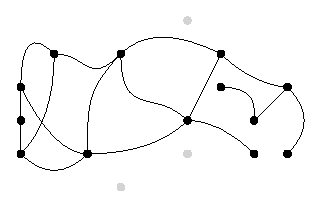
\includegraphics[width=200pt]{images/vertex-cover-3.eps}
    }
    \only<2->{
        \includegraphics[width=200pt]{images/vertex-cover-4.eps}
    }

    \only<1>{
        \questionbox{
            \centering
            Wie lässt sich die Instanz vereinfachen?
        }
    }
    
    \only<2>{
        \answerbox{
            \centering
            Wenn ein Knoten Knotengrad min. $k+1$ hat, ist er in der Menge enthalten.    
        }
    }

    \visible<1->{
        \tikz[overlay, remember picture] \node[xshift=-28mm, yshift=-14mm] at (current page.north east) {
            \begin{StickyNote}
                Instanzen äquivalent, wenn Ja-Instanz auf Ja-Instanz abgebildet wird.
            \end{StickyNote}
        };
    }

    \only<3->{
        \begin{grayblock}{2. Reduktionsregel}
            Ist $(G, k)$ eine $k$-Vertex-Cover Instanz mit Parameter $k$ und $v \in V(G)$ Knoten mit $deg(v) \geq k+1$, so ist $(G-v, k-1)$ eine äquivalente Instanz.
        \end{grayblock}
    }

    \only<4>{
        \raggedright
        \textbf{Beweis:}
        \\
        \enquote{$\Rightarrow$}:
        \\
        Ist G eine Ja-Instanz, so existiert Menge $M$ als Vertex Cover.
        \\
        Dann hat G-v das Vertex Cover $M' = M\setminus{\{v\}}$. Insbesondere ist $|M'| = |M| - |\{v\}| \leq k - |\{v\}| = k - 1  $
    }

    \only<5->{
        \raggedright
        \textbf{Beweis:}
        \\
        \enquote{$\Leftarrow$}:
        \\
        Ist $G-v$ eine Ja-Instanz, so existiert Menge $M'$ als Vertex Cover.
        Wird nun $v$ hinzugefügt und so $G$ erzeugt, werden die neu hinzugefügten Kanten durch $v$ abgedeckt. G hat das Vertex Cover $M = M' \cup \{v\}$.
    }
\end{frame}

\begin{frame}[t]{}
    \vspace*{\fill}
    \centering

    \vspace{10pt}
    \only<1>{
        \includegraphics[width=200pt]{images/vertex-cover-5.eps}
    }
    \only<2->{
        \includegraphics[width=200pt]{images/vertex-cover-4.eps}
    }

    \only<1>{
        \questionbox{
            \centering
            Wie lässt sich die Instanz vereinfachen?
        }
    }
    
    \only<2>{
        \answerbox{
            \centering
            Hat der Graph nach erschöpfnender Anwendung von Regel 2 mehr als $k^2$ Kanten, ist $G$ eine Nein-Instanz.
        }
    }

    \visible<1->{
        \tikz[overlay, remember picture] \node[xshift=-28mm, yshift=-14mm] at (current page.north east) {
            \begin{StickyNote}
                Instanzen äquivalent, wenn Ja-Instanz auf Ja-Instanz abgebildet wird.
            \end{StickyNote}
        };
    }

    \only<3->{
        \begin{grayblock}{3. Reduktionsregel}
            Ist $(G, k)$ eine $k$-Vertex-Cover Instanz die durch erschöpfende Anwendung der 2. Reduktionsregel entstanden ist mit $|E(G)| > k^2$, ist G eine Nein-Instanz.
        \end{grayblock}
    }

    \only<4>{
        \raggedright
        \textbf{Beweis:}
        \\
        \enquote{$\Rightarrow$}:
        \\
        Nach erschöpfender Anwendung der 2. Regel hat jeder Knoten v $deg(v) \leq k$.
        \\
        Eine Vertex-Cover von $k$ Knoten kann damit maximal $k^2$ Kanten abdecken.
    }
\end{frame}

\begin{frame}{Zwischenergebnis}
    \begin{grayblock}{1. Reduktionsregel}
        Ist $(G, k)$ eine $k$-Vertex-Cover Instanz mit Parameter $k$ und $U$ die Menge der isolierten Knoten in G, \\ so ist $(G-U, k)$ eine äquivalente Instanz.
    \end{grayblock}
    \begin{grayblock}{2. Reduktionsregel}
        Ist $(G, k)$ eine $k$-Vertex-Cover Instanz mit Parameter $k$ und $v \in V(G)$ Knoten mit $deg(v) \geq k+1$, so ist $(G-v, k-1)$ eine äquivalente Instanz.
    \end{grayblock}
    \begin{grayblock}{3. Reduktionsregel}
        Ist $(G, k)$ eine $k$-Vertex-Cover Instanz die durch erschöpfende Anwendung der 2. Reduktionsregel entstanden ist mit $|E(G)| > k^2$, ist G eine Nein-Instanz.
    \end{grayblock}

    \visible<2>{
        \vspace{5pt}
        \centering
        \textbf{
            Wie sieht der Graph nach erschöpfnender Anwendung der Reduktionsregeln aus?
        }
    }
\end{frame}

\begin{frame}{Ein Problemkern für VERTEX-COVER}
    \begin{greenblock}{Satz}
        Eine k-VERTEX-COVER Instanz (G, k) reduziert sich nach erschöpfender Anwendung der Reduktionsregeln 1 - 3 auf eine Größe in \BigO{k^2}.
    \end{greenblock}

    \visible<2->{
        \raggedright
        \textbf{Beweis:}
        \\
        Sei $\tilde{G}$ der Graph der aus einer k-VERTEX-COVER Instanz nach ershöpfender Anwendung der Reduktionsregeln 1-3 entstanden ist.
        \\
        zu zeigen: $|V(\tilde{G})| \in \BigO{k^2}$
        \\
        \begin{itemize}
            \item Durch Anwendung von 1. besitzt $\tilde{G}$ keine isolierten Knoten.
            \\
            (also ist jeder Knoten zu min. einer Kante adjazent)
            \item Durch Anwendung von 3. (unter Zuhilfenahme von 2.) existieren max. $k^2$ viele Kanten.
            
            $\Rightarrow$ Damit existieren maximal $2k^2$ viele Knoten.
        \end{itemize}
    }

    \visible<3->{
        \centering
        \textbf{Damit ist die Problemgröße nur noch vom Parameter abhängig!}
    }

    \visible<4->{
        \centering
        \textbf{Alle Reduktionen sind in polynomieller Zeit durchführbar!}
    }

\end{frame}

\begin{frame}[t]{Problemkerne \& Problemkernreduktion}
    \begin{itemize}
        \item \textbf{Ziel:} gerade gesehene Konzepte verallgemeinern und formalisieren
    \end{itemize}

    \begin{blueblock}{Problemkern \& Problemkernreduktion}
        Sei $ P \subseteq (\Sigma^*, \N) $ ein parametrisiertes Problem über einem endlichen Alphabet $\Sigma$.
        \\
        Es bezeichne $|I|$ die (Eingabe-)Größe einer Probleminstanz $I \in (\Sigma^*, \N)$.
        \\
        Eine Problemkernreduktion $ \Phi: (\Sigma^*, \N) \rightarrow (\Sigma^*, \N) $ ist eine Funktion sodass:
        \begin{itemize}
            \item $(I, k) \in P \iff (I', k') := \Phi(I, k) \in P $
            \item $|I'| \leq f(k)$ für eine beliebige Funktion $f: \N \rightarrow \N$
            \item $f$ ist in Polynomialzeit berechenbar
        \end{itemize}
        \vspace{20pt}
        $ \Phi(I, k) $ heißt \textbf{Problemkern} von $(I, k)$.
    \end{blueblock}
\end{frame}

\end{document} 
